\documentclass[a4paper,12pt]{report}

\usepackage[vietnamese]{babel}
\usepackage[utf8]{inputenc, vietnam}
\usepackage[a4paper,margin=24mm]{geometry}
\usepackage[skip=10pt plus1pt, indent=20pt]{parskip}
\usepackage[colorlinks=true,allcolors=blue,urlcolor=magenta]{hyperref}

\usepackage{caption}
\usepackage{indentfirst,setspace,subcaption}
\usepackage{amsmath,amssymb,graphicx,xcolor,url}
\usepackage{fancyhdr,tocbasic,titlesec,minted,listings}

\renewcommand{\thesection}{\arabic{section}}

% Header and footer styling
\pagestyle{fancy}
\setlength{\headheight}{18pt}
\fancyhf{}
\fancyhead[R]{\nouppercase\rightmark\hfill~Báo cáo đồ án Socket}
\fancyfoot[C]{\hfill\thepage\hfill}

% TOC styling
\DeclareTOCStyleEntry[
  indent=12pt,
  level=1
]{largetocline}{section}

% Title page data
\title{Báo cáo đồ án Socket}
\author{\begin{tabular}{r c}
  Ngô Nguyễn Thế Khoa & 23127065\\
  Hình Diễm Xuân      & 23127524\\
  \end{tabular}}

\date{Ngày 25 tháng 6 năm 2024}
% \date{June 25, 2024}
% \date{\today}

\begin{document}

% Title page and TOC
\thispagestyle{empty}
\begin{titlepage}
	\begin{center}
		\makeatletter
		\newcommand{\HRule}{\rule{\linewidth}{0.4mm}}

		\textsc{\LARGE Đại học Quốc gia\\Thành phố Hồ Chí Minh}\\[1.5cm]
		\textsc{\Large Trường Đại học Khoa học Tự nhiên}\\[0.5cm]
		\textsc{\Large khoa công nghệ thông tin}\\[1.5cm]

		{\HRule}\\[1cm]
		{\huge \bfseries \@title}\\[0.5cm]
		{\HRule}\\[2cm]

		\textsc{\large CSC10008 -- MẠNG MÁY TÍNH}\\[0.5cm]

		\vfill\vfill\vfill

		{\large \@author}\\[1.5cm]
		{\large \@date}
		\makeatother
	\end{center}
\end{titlepage}
\tableofcontents\thispagestyle{empty}

% Report contents
\pagebreak
\section{Thông tin nhóm}
\begin{itemize}
  \item \textbf{Môn:} Mạng máy tính
  \item \textbf{Lớp học phần:} 23CLC09
  \item \textbf{Giảng viên hướng dẫn:} Lê Hà Minh
  \item \textbf{Thành viên:}
        \begin{center}
          \renewcommand{\arraystretch}{1.5}
          \begin{tabular}{|c|l|l|c|l|}
            \hline
            \textbf{STT} & \textbf{Họ và tên}  & \textbf{MSSV} & \textbf{Email}                                                       & \textbf{Vai trò} \\\hline
            1            & Ngô Nguyễn Thế Khoa & 23127065      & \href{mailto:nntkhoa23@clc.fitus.edu.vn}{nntkhoa23@clc.fitus.edu.vn} & Trưởng nhóm      \\\hline
            2            & Hình Diễm Xuân      & 23127524      & \href{mailto:hdxuan23@clc.fitus.edu.vn}{hdxuan23@clc.fitus.edu.vn}   & Thành viên       \\\hline
          \end{tabular}
        \end{center}
  \item \textbf{Công cụ hỗ trợ:}
        \begin{itemize}
          \item \href{https://git-scm.com/}{\textbf{Git}}, \href{https://github.com/}{\textbf{GitHub}}
          \item \href{https://www.canva.com/}{\textbf{Canva}}
          \item \href{https://docs.google.com/spreadsheets/}{\textbf{Google Sheets}}
        \end{itemize}
\end{itemize}

\pagebreak
\section{Bảng đánh giá mức độ hoàn thành}
\begin{center}
  \renewcommand{\arraystretch}{1.5}
  \begin{tabular}{|c|p{\dimexpr0.6\linewidth-\tabcolsep}|c|}
    \hline
    \textbf{STT} & \textbf{Yêu cầu}                                                                                         & \textbf{Tiến độ}                        \\\hline
    \multicolumn{3}{|c|}{\textbf{Phần I}}                                                                                                                                                \\\hline
    1            & Client có thể nhận được danh sách các file từ Server và ctrl-c                                           & 100\%             \\\hline
    2            & Client có thể nhận lần lượt từng file thành công từ Server. Server có thể gửi file thành công tới Client & 100\%             \\\hline
    3            & Hiển thị percent download file và phát hiện những file cần download tiếp theo                            & 100\%             \\\hline
    \multicolumn{3}{|c|}{\textbf{Phần II}}                                                                                                                                               \\\hline
    4            & Client có thể nhận được danh sách các file từ Server và ctrl-c                                           & 100\%             \\\hline
    5            & 2s quét file input.txt 1 lần                                                                             & 100\%             \\\hline
    6            & Hiển thị phần trăm download files                                                                       & 100\%             \\\hline
    7            & Client có thể nhận files thành công từ Server. Tập tin sau khi download phải đúng và đủ dung lượng       & 100\%             \\\hline
    8            & Độ ưu tiên CRITICAL, HIGH, NORMAL                                                                        & 100\%             \\\hline
    \multicolumn{3}{|c|}{\textbf{Tổng kết báo cáo}}                                                                                                                                      \\
    \multicolumn{3}{|c|}{\textsl{Hoàn thành 100\% yêu cầu đồ án}}                                                                                                                        \\
    \multicolumn{3}{|c|}{\textsl{Không xảy ra lỗi khi vận hành chương trình}}                                                                                                            \\\hline
  \end{tabular}
\end{center}

\pagebreak
\section{Nội dung}
\subsection{Thông tin chung về đồ án:}
\begin{enumerate}
  \item \textbf{Tên đồ án:} Lập trình Socket
  \item \textbf{Môi trường lập trình:} Visual Studio Code, Windows
  \item \textbf{Ngôn ngữ lập trình:} Python
  \item \textbf{Danh sách thư viện chuẩn được sử dụng (standard libs)}
        \begin{itemize}
          \item \verb|argparse| - parse command line arguments
          \item \verb|datetime| - parse datetime with custom format
          \item \verb|enum| - usage of enum type
          \item \verb|json| - data serialization
          \item \verb|os| - file operations
          \item \verb|pathlib| - usage of filesystem path
          \item \verb|re| - usage of regex
          \item \verb|socket| - creating sockets
          \item \verb|sys| - rendering progress bar (pure progress bar)
          \item \verb|threading| - handling multiple clients
          \item \verb|time| - time operations
          \item \verb|typing| - usage of generic type
          \item \verb|unittest| - testing functions
        \end{itemize}
  \item \textbf{Danh sách thư viện bổ sung được sử dụng (external libs)}
        \begin{itemize}
          \item \verb|customtkinter| - making GUI
          \item \verb|python-dotenv| - load configs from \verb|.env| files
          \item \verb|rich| - rendering more beautiful console progress bar
          \item \verb|watchdog| - watching file changes
        \end{itemize}
  \item  \textbf{Giao thức trao đổi giữa Client và Server:} Giao thức TCP
\end{enumerate}

\subsection{Một số lưu ý}
\begin{flushleft}
  \begin{itemize}
    \item Cần cấu hình file \verb|.env| trước khi chạy chương trình (cấu hình cho Server và Client)
    \item Tải thư viện bổ sung bằng lệnh \verb|pip install -r requirements.txt| (trong thư mục \verb|Source|)
    \item Chạy Server trước khi chạy bất kì Client nào
    \item Cần chạy một Socket Server khác với địa chỉ đã được dùng trước đó, nếu không sẽ không thể tạo được một Socket Server mới
  \end{itemize}
\end{flushleft}

\subsection{Cấu trúc đồ án}
\begin{flushleft}
  \begin{description}
    \item[(Source):]
          Thư mục chứa mã nguồn của chương trình\\
          \begin{description}
            \item[(app):]
                  Thư mục chứa mã nguồn của Server và Client
                  \begin{description}
                    \item[(client):]
                          Thư mục ứng dụng hoạt động (có thể tùy chỉnh)\\
                          \begin{description}
                            \item[(downloads):] Thư mục chứa các file đã tải về (đường dẫn mặc định)
                            \item[input.txt:] File chứa danh sách file cần tải về (đường dẫn mặc định)
                          \end{description}
                    \item[(server):]
                          Thư mục ứng dụng hoạt động (có thể tùy chỉnh)\\
                          \begin{description}
                            \item[(resources):] Thư mục chứa các file có thể tải về (đường dẫn mặc định)
                            \item[resources.json:] File chứa danh sách file có thể tải về (tự động tạo và cập nhật)
                          \end{description}
                  \end{description}
            \item[(classes):] Thư mục chứa các class hỗ trợ cho Server và Client
            \item[(shared):] Thư mục chứa các biến chung cho Server và Client
            \item[(tests):] Thư mục chứa các chương trình dùng để test hàm
            \item[(utils):] Thư mục chứa các hàm hỗ trợ cho Server và Client
            \item[.env:] File cấu hình cho Server và Client
            \item[requirements.txt:] File chứa danh sách thư viện cần cài đặt
            \item[server.py:] Mã nguồn của Server
            \item[client.py:] Mã nguồn của Client
          \end{description}
    \item[Report.pdf:] Báo cáo đồ án
  \end{description}
\end{flushleft}

\subsection{Nguyên lí hoạt động - Kịch bản giao tiếp:}
\begin{itemize}
  \item \textbf{Giao thức kết nối:} TCP
  \item \textbf{Kịch bản giao tiếp:}
        \begin{description}
          \item \textbf{Client:}
                \begin{itemize}
                  \item \verb|help|: Lệnh hiển thị danh sách các lệnh có thể sử dụng
                  \item \verb|quit|: Lệnh thoát chương trình, được gửi khi có tín hiệu kết thúc phiên chạy (Ctrl + C hoặc lệnh \verb|quit|)
                  \item \verb|list|: Lệnh hiển thị danh sách các file có thể tải về từ Server
                        \begin{enumerate}
                          \item Chờ nhận dữ liệu từ Server và hiển thị danh sách file
                                \begin{itemize}
                                  \item Danh sách các file được gửi dưới dạng\\`\verb|LIST {sep} {filename} {sep} {file_sz} {sep}|'
                                  \item Nếu trong quá trình nhận dữ liệu, nhận được lệnh \verb|terminate| từ Server \(\Rightarrow \) Kết thúc phiên chạy
                                \end{itemize}
                        \end{enumerate}
                  \item \verb|file|: Lệnh tải file được gửi từ Client để thiết lập quá trình tải file
                        \begin{enumerate}
                          \item Chờ nhận lệnh \verb|accept| từ Server
                          \item Nếu nhận được lệnh \verb|accept|, tiến hành tải file bằng cách gửi thông điệp dưới dạng\\`\verb|DATA {sep} {filename} {sep} {chunk_sz} {sep}|'
                          \item Chờ nhận dữ liệu từ Server và lưu vào file
                                \begin{itemize}
                                  \item Nếu trong quá trình nhận dữ liệu, nhận được lệnh \verb|done| từ Server \(\Rightarrow \) Tải file thành công
                                  \item Nếu trong quá trình nhận dữ liệu, nhận được lệnh \verb|terminate| từ Server \(\Rightarrow \) Kết thúc phiên chạy
                                \end{itemize}
                        \end{enumerate}
                \end{itemize}
          \item \textbf{Server:}
                \begin{itemize}
                  \item \verb|done|: Lệnh thông báo tải file thành công
                  \item \verb|invalid|: Lệnh thông báo lệnh nhận được từ Client không hợp lệ
                  \item \verb|terminate|: Lệnh ngắt kết nối đến tất cả Client (được gửi đi khi Server nhận tín hiệu kết thúc phiên chạy)
                  \item \verb|accept|: Lệnh thông báo Server hoàn tất thiết lập tải file từ Client
                        \begin{enumerate}
                          \item Chờ nhận thông điệp từ Client và tiến hành tải file
                                \begin{itemize}
                                  \item Gửi dữ liệu file dưới dạng \verb|bytes| cho Client
                                  \item Nếu trong quá trình nhận dữ liệu, nhận được lệnh \verb|quit| từ Client \(\Rightarrow \) Kết thúc phiên chạy của Client Socket tương ứng bên Server
                                \end{itemize}
                        \end{enumerate}
                \end{itemize}
        \end{description}
  \item \textbf{Kiểu dữ liệu của thông điệp:} kiểu \verb|string|, gửi bằng lệnh \verb|send, sendall| và nhận bằng lệnh \verb|recv| theo FORMAT được quy ước
  \item \textbf{Sơ đồ minh họa một phần quá trình giao tiếp giữa Client và Server sử dụng giao thức TCP:}
        \begin{figure}[ht]
          \centering
          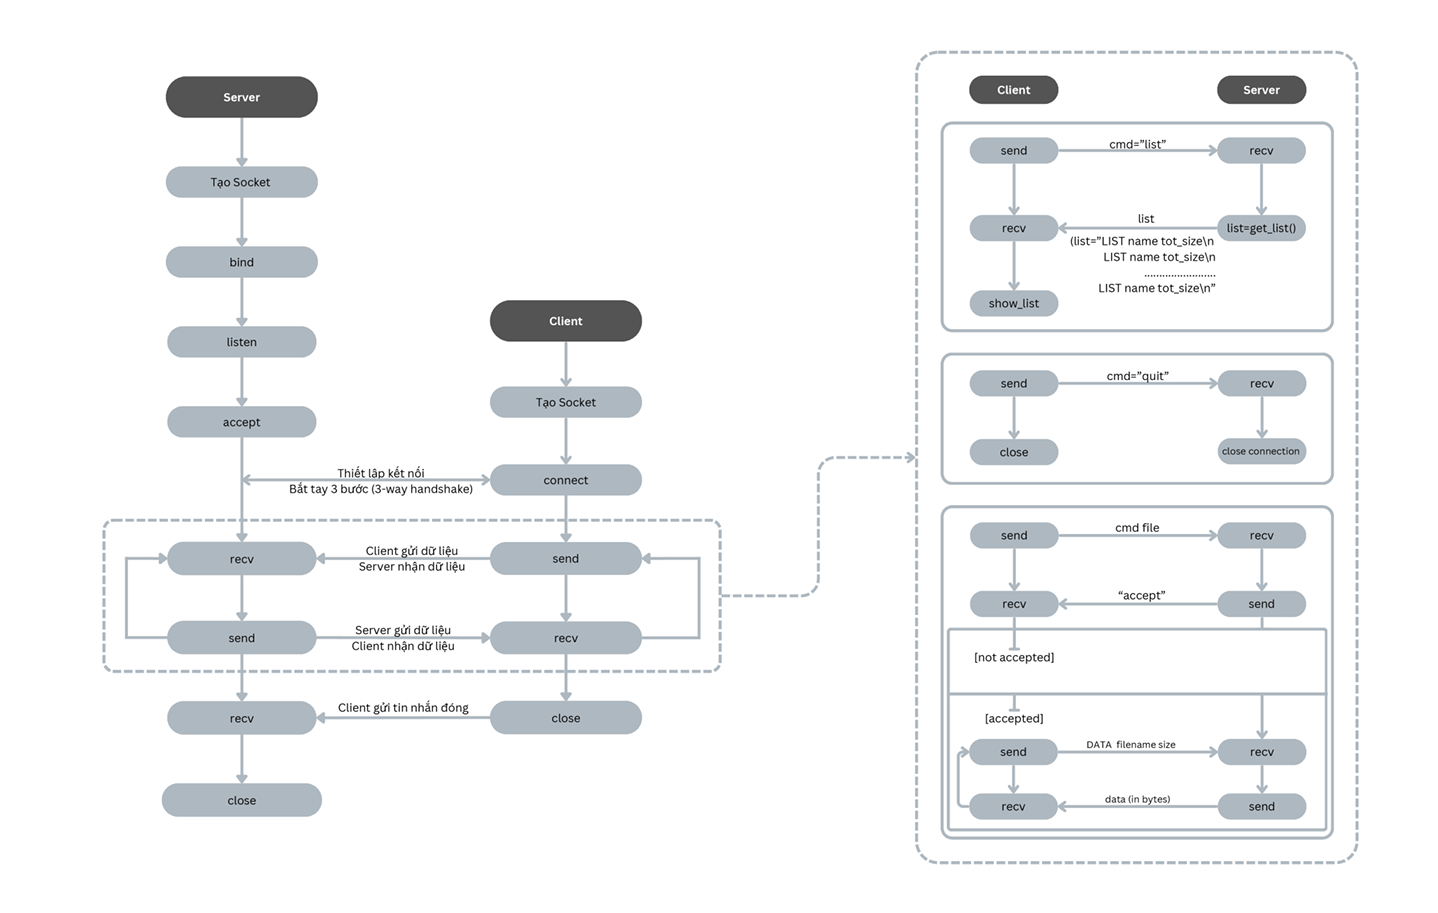
\includegraphics[width=1\textwidth]{Screenshots/diagram.png}
          \caption{Sơ đồ minh họa kịch bản giao tiếp}\label{fig:diagram}
        \end{figure}
\end{itemize}

\pagebreak
\section{Các tính năng chương trình}
\subsection{Các tính năng cơ bản}
\begin{enumerate}
  \item Server phục vụ đồng thời nhiều Client cùng lúc.
  \item Client nhận được danh sách tài nguyên từ Server.
  \item Thêm file mới vào danh sách  tải và thêm vào độ ưu tiên tải nếu muốn (Phần 2).
  \item Duyệt file mỗi khi tải xong từng file (Phần 1) và duyệt file mỗi 2 giây (Phần 2).
  \item Mỗi Client chỉ dùng duy nhất một kết nối để download tuần tự các phần nhỏ xen kẽ của từng file từ server (Phần 2).
  \item Hiển thị thanh tiến độ tải.
  \item Khi Client bấm `Ctrl + C' thì chương trình client đóng kết nối đến Server và kết thúc chương trình.
  \item Khi Server bấm `Ctrl + C' thì kết thúc phiên chạy Server và đóng kết nối tới các Client.
\end{enumerate}
\subsection{Các tính năng bổ sung}
\begin{enumerate}
  \item Giao diện Console cơ bản cho Server.
  \item Giao diện Console cơ bản và nâng cấp cho Client.
  \item Giao diện người dùng đồ họa (GUI) cho Server và Client.
  \item Tự động cập nhật danh sách tài nguyên trên Server nếu có bất kì sự thay đổi nào (đổi tên file, xóa file, \ldots).
  \item Sử dụng \verb|command line arguments| để chạy bất kì phiên bản nào (sử dụng GUI/Console, chạy phần 1) của Server và Client một cách thuận tiện.
        \begin{itemize}
          \item \verb|py server.py --part1|: Chạy Server với yêu cầu phần 1.
          \item \verb|py client.py --part1|: Chạy Client với yêu cầu phần 1.
          \item \verb|py server.py --gui|: Chạy Server với giao diện người dùng đồ họa.
          \item \verb|py client.py --gui|: Chạy Client với giao diện người dùng đồ họa.
          \item \verb|py client.py --rich|: Chạy Client với giao diện console nâng cấp.
          \item Các lệnh trên có thể kết hợp với nhau mà không gây xung đột.
        \end{itemize}
\end{enumerate}
\subsection{Các trường hợp đặc biệt khi chạy chương trình}
\begin{enumerate}
  \item Khởi tạo một Socket Server mới với địa chỉ đã được sử dụng sẽ không thành công.
  \item Trong quá trình tải file, nếu Client bấm `Ctrl + C' thì kết thúc phiên chạy của Client đó và Server cũng sẽ ngắt kết nối với Client đó.
  \item Trong quá trình tải file, nếu Server bấm `Ctrl + C' thì kết thúc phiên chạy của Server và ngắt kết nối với tất cả Client, đồng thời các file đang tải cũng sẽ dừng tải và Client kết thúc chương trình.
\end{enumerate}

\pagebreak
\section{Hướng dẫn sử dụng tính năng chương trình}
\begin{description}
  \item \textbf{Chuẩn bị:} Cấu hình file \verb|.env| trước khi chạy chương trình (cấu hình cho Server và Client) và tải thư viện bổ sung bằng lệnh \verb|pip install -r requirements.txt| (trong thư mục \verb|Source|).
        \begin{itemize}
          \item \textbf{Server:}
                \begin{itemize}
                  \item \verb|HOST|: Địa chỉ IP của Server
                  \item \verb|PORT|: Cổng kết nối của Server
                  \item \verb|SERVER_RESOURCES_PATH|: Đường dẫn chứa tài nguyên có thể tải về
                \end{itemize}
          \item \textbf{Client:}
                \begin{itemize}
                  \item \verb|HOST|: Địa chỉ IP của Server
                  \item \verb|PORT|: Cổng kết nối của Server
                  \item \verb|CLIENT_DOWNLOADS_PATH|: Đường dẫn chứa tài nguyên đã tải về
                  \item \verb|CLIENT_REQUEST_INPUT|: Đường dẫn file chứa danh sách file cần tải về
                \end{itemize}
        \end{itemize}
  \item \textbf{Bước 1:}
        \begin{itemize}
          \item Chạy file \verb|server.py| bằng lệnh \verb|py server.py|, lúc này một Socket Server sẽ chạy và chờ các kết nối từ Client.
          \item Chạy file \verb|client.py| bằng lệnh \verb|py client.py| khởi tạo một Socket Client và tự động kết nối đến Server.
        \end{itemize}
  \item \textbf{Bước 2:} Sau khi Client kết nối thành công, Server sẽ hiển thị địa chỉ của Client đã kết nối và gửi đi danh sách tài nguyên có thể tải về cho Client.
  \item \textbf{Bước 3:} Nhập những file muốn tải vào \verb|input.txt| trong đường dẫn của ứng dụng Client (mặc định ở \verb|Source/app/client/input.txt|). Client sẽ tự động đọc (sau khi tải xong file đối với Phần 1 và mỗi 2s đối với Phần 2) và tải file trong danh sách theo mức độ ưu tiên được quy ước từ trước.\\ \\
        Ngoài ra còn có thể nhập lệnh bằng \verb|console| (Client) với quy tắc giao tiếp:
        \begin{itemize}
          \item \verb|"help", "h"|: Hiển thị danh sách các lệnh có thể dùng.
          \item \verb|"quit", "q"|: Ngắt kết nối với Server và kết thúc chương trình.
          \item \verb|"list", "l"|: Gửi yêu cầu lấy danh sách các file có thể tải về từ Server sau đó nhận dữ liệu và hiển thị danh sách này.
          \item \verb|"file", "f"|: Tiến hành tải file từ Server dựa trên dữ liệu trong file \verb|input.txt|.
        \end{itemize}
  \item \textbf{Bước 4:} Ngắt kết nối bằng cách \verb|Ctrl+C| (có thể thực hiện ở cả Server và Client) hoặc nhập lệnh \verb|"q"| (chỉ ở Client).
\end{description}

% \pagebreak
\section{Bảng phân công việc}
\begin{center}
  \renewcommand{\arraystretch}{1.5}
  \begin{tabular}{|c|p{\dimexpr0.6\linewidth-2\tabcolsep}|c|}
    \hline
    \textbf{STT} & \textbf{Công việc}                                                                                         & \textbf{Người thực hiện} \\\hline
    1            & Viết báo cáo                                                                             & Khoa, Xuân               \\\hline
    2            & Kiểm thử phần mềm (kiểm tra các tính năng và rà soát lỗi)                                     & Xuân               \\\hline
    3            & Thiết kế mẫu giao diện                                                                         & Xuân               \\\hline
    4            & Tích hợp commandline interface                                                                & Xuân               \\\hline
    5            & Vẽ biểu đồ kịch bản giao tiếp giữa Client và Server                                                & Xuân               \\\hline
    6            & Lấy danh sách tài nguyên và hiển thị danh sách file hiện có bên Server       & Khoa             \\\hline
    7            & Lấy kích thước, đường dẫn tới file                                                                       & Khoa             \\\hline
    8            & Lấy danh sách file cần tải từ input.txt (Client)                                             & Khoa             \\\hline
    9            & Lấy dữ liệu, kích thước, đường dẫn của các tài nguyên (Server)                                       & Khoa             \\\hline
    10           & Trích xuất thông tin từ file input.txt, xử lí độ ưu tiên tải (CRIT, HIGH, NORM)                                    & Khoa             \\\hline
    11           & Tạo các thành phần (khung, thanh cuộn, khung chữ, check box, ...) cho giao diện đồ họa                               & Khoa             \\\hline
    12           & Tạo tên nhãn, ghi chữ, tạo nút cho giao diện                                                      & Khoa             \\\hline
    13           & Tạo thanh tiến trình, bảng điều khiển, cấu hình khung cho giao diện                           & Khoa             \\\hline
    14           & Ghi log vào console và file để theo dõi quá trình thực thi                & Khoa             \\\hline
    15           & Theo dõi sự thay đổi trong thư mục "resources"~(thêm mới, chỉnh sửa file tài nguyên) và tiến hành cập nhật file `resources.json` (file chứa thông tin về các tài nguyên như tên file, dung lượng và đường dẫn) & Khoa             \\\hline
    16           & Xử lí các exception (ngoại lệ)                & Khoa             \\\hline
    17           & Gửi tín hiệu để xác định trạng thái kết nối (Server và Client)         & Khoa             \\\hline
    18           & Xử lí thoát và dừng khi có tín hiệu tương ứng              & Khoa             \\\hline
    19           & Bộ đếm ngược thời gian chờ kết nối đến Server                & Khoa             \\\hline
    \end{tabular}
\pagebreak
\begin{tabular}{|c|p{\dimexpr0.6\linewidth-2\tabcolsep}|c|}
    \hline
    \textbf{STT} & \textbf{Công việc} & \textbf{Người thực hiện} \\\hline
    20           & Xử lí tải file                 & Khoa             \\\hline
    21           & Tạo giao diện (gui) cho Client               & Khoa             \\\hline
    22           & Tạo giao diện (gui) cho Server               & Khoa             \\\hline
    23           & Server xử lí tín hiệu từ Client và hoạt động theo lệnh commandline               & Khoa             \\\hline
    24           & Client nhận dữ liệu từ Server theo từng chunk đã xử lí             & Khoa
    \\\hline
  \end{tabular}
\end{center}

\pagebreak
\section{Ảnh chụp màn hình}
\subsection{Console UI}
\begin{figure}[ht]
  \centering
  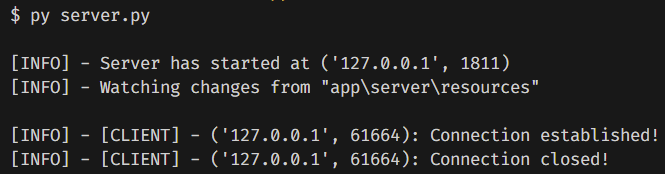
\includegraphics[width=0.7\textwidth]{Screenshots/server-console.png}
  \caption{Giao diện Server (Console)}\label{fig:server-console}
\end{figure}
\begin{figure}[ht]
  \centering
  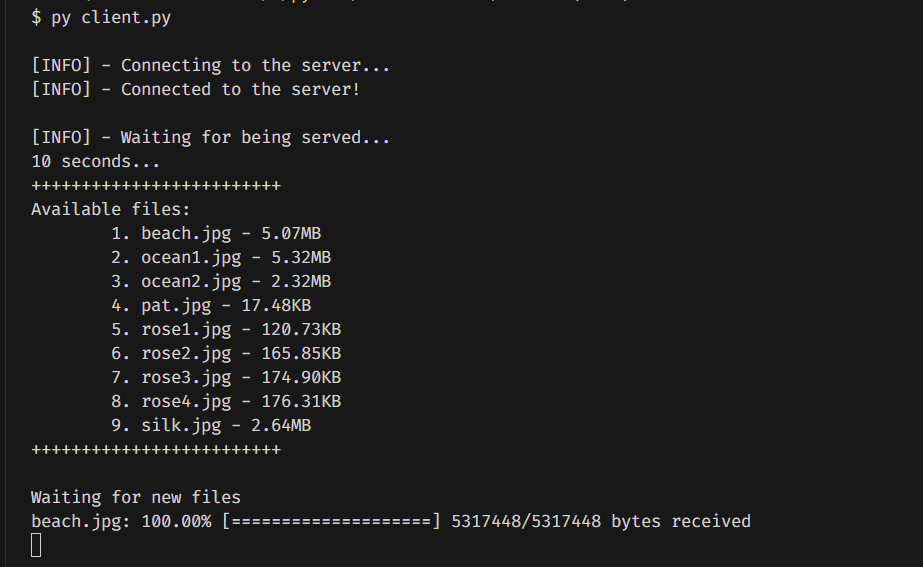
\includegraphics[width=0.7\textwidth]{Screenshots/client-console.png}
  \caption{Giao diện Client (Console)}\label{fig:client-console}
\end{figure}
\begin{figure}[ht]
  \centering
  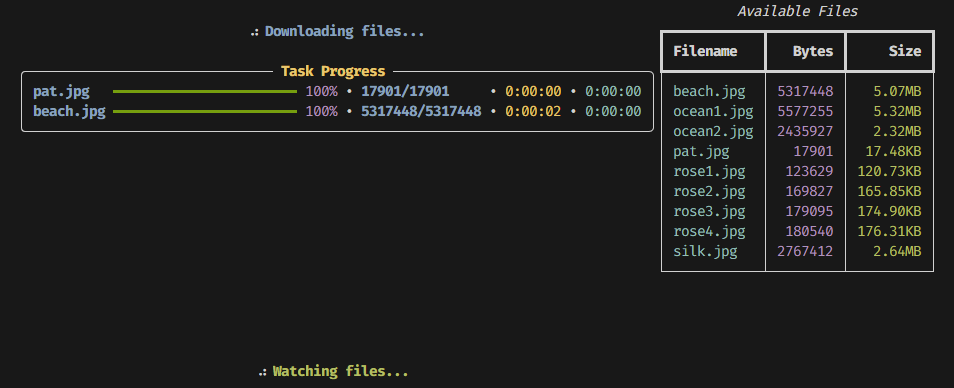
\includegraphics[width=0.7\textwidth]{Screenshots/client-rich.png}
  \caption{Giao diện Client (Rich)}\label{fig:client-rich}
\end{figure}

\pagebreak
\subsection{Graphical User Interface (GUI)}
\begin{figure}[ht]
  \centering
  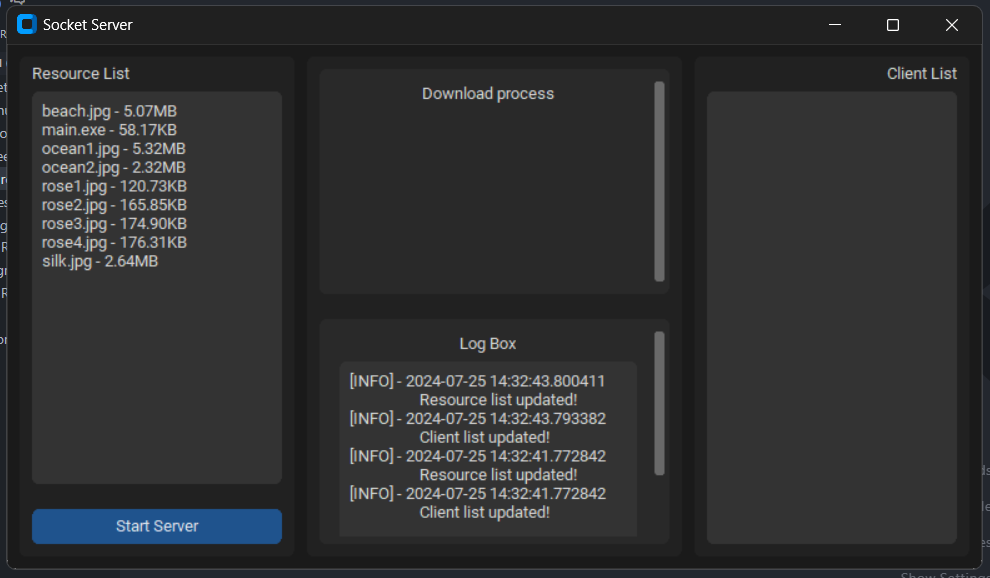
\includegraphics[width=0.7\textwidth]{Screenshots/server-gui.png}
  \caption{Giao diện Server (GUI)}\label{fig:server-gui}
\end{figure}
\begin{figure}[ht]
  \centering
  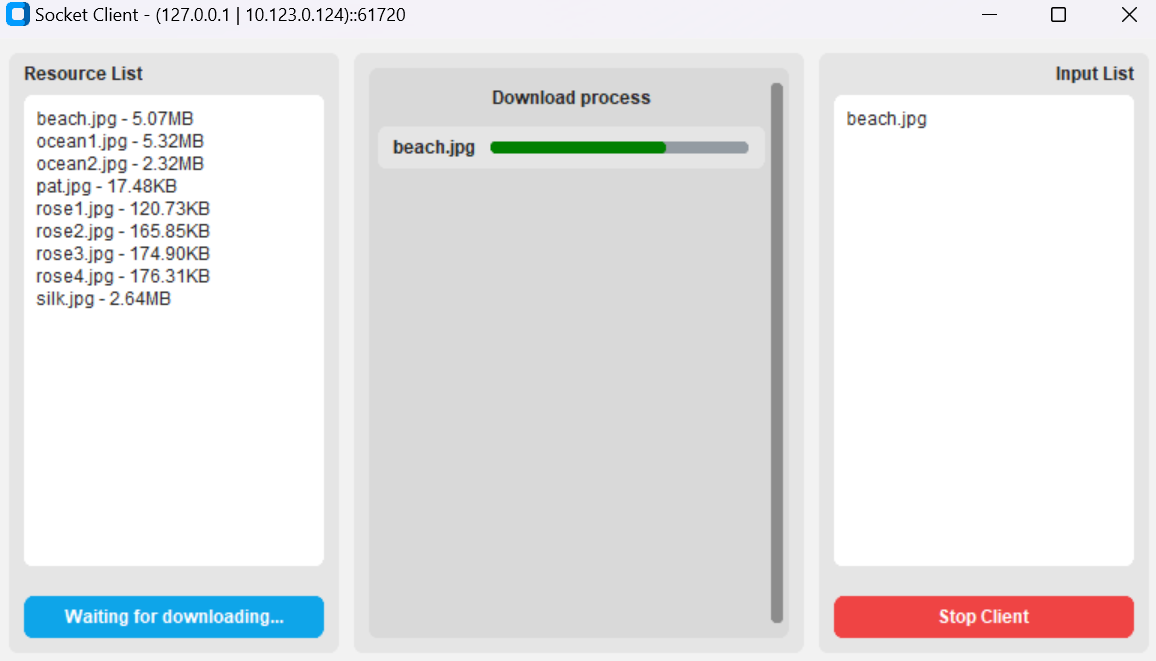
\includegraphics[width=0.7\textwidth]{Screenshots/client-gui.png}
  \caption{Giao diện Client (GUI)}\label{fig:client-gui}
\end{figure}

% References
\pagebreak
\section{Nguồn tham khảo}
\begin{enumerate}
  \item \href{https://realpython.com/intro-to-python-threading}{Python Threading}
  \item \href{https://realpython.com/python-sockets/#handling-multiple-connections}{Python Socket Programming}
  \item \href{https://stackoverflow.com/questions/47847392/keyboard-interrupt-sockets-and-threads}{Keyboard interrupt sockets and threads}
  \item \href{https://github.com/hadis98/FTP-Client-Server-Python-Socket-Programming}{Socket FTP}
\end{enumerate}

\end{document}